\section{Effect of transitioning}
The basic specification is given by:
\beqn
	y_{iot}&=&\lambda_o +\beta_1 e_i+\beta_2 1_{\{t>transition\_time\}}+\beta_3 e_i\times 1_{\{t>transition\_time\}}
\eeqn
where $\lambda_o$ denotes occupation fixed-effects, $e_i$ is an education-level dummy. xpectation: $\beta_1\neq0$, $\beta_2=\beta_3=0$. I try four different definitions of the transition year:
\bitem
	\item \textit{First out}: first year out of the initial category.
	\item \textit{Last out:} last year in initial category + 1.
	\item \textit{First in: } first year in final category.
	\item \textit{Last in:} latest year of transition into final category + 1.
\eitem

\begin{figure}[!h]
\caption{Number of transitioned occupations by transition type}
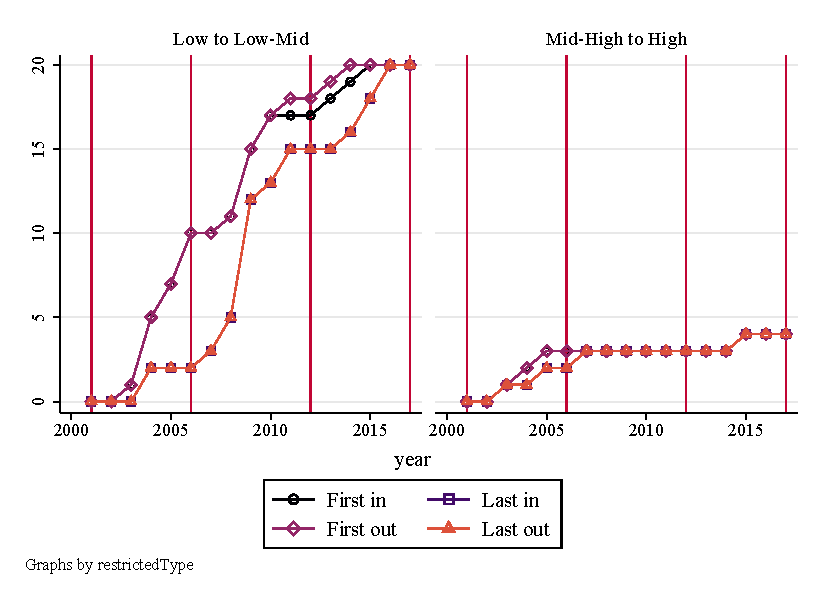
\includegraphics[width=\textwidth]{../output/transition_timeline}
\par \begin{minipage}[h]{\textwidth}{\scriptsize\textbf{Note:} Transitions are defined as the union of 3-3-3, 4-2-3 and 2-4-3. Vertical lines indicate years for which I have SES data. Figure generated on 12 Jun 2020 at 15:09:22. Figure generated using the dofile 4\_lfsAnalysis/transition\_time\_graphs.do.}\end{minipage}
\end{figure}


\FloatBarrier


{ \footnotesize
	\begin{center}
\begin{threeparttable}[!h]
\caption{Dependent variable: analytical skill}
\begin{tabular}{lcccccccc}
\toprule
\toprule
&\multicolumn{1}{c}{\textbf{}}&\multicolumn{1}{c}{\textbf{}}&\multicolumn{1}{c}{\textbf{}}&\multicolumn{1}{c}{\textbf{}}&\multicolumn{1}{c}{\textbf{}}&\multicolumn{1}{c}{\textbf{}}&\multicolumn{1}{c}{\textbf{}}&\multicolumn{1}{c}{\textbf{}} \\
\textbf{Regressor}&\multicolumn{1}{c}{(1)}&\multicolumn{1}{c}{(2)}&\multicolumn{1}{c}{(3)}&\multicolumn{1}{c}{(4)}&\multicolumn{1}{c}{(5)}&\multicolumn{1}{c}{(6)}&\multicolumn{1}{c}{(7)}&\multicolumn{1}{c}{(8)} \\
\midrule
\textit{Low to Low-Mid} \\
Mid                 &       0.032         &       0.020         &       0.039\sym{*}  &       0.026         &       0.032         &       0.020         &       0.039\sym{*}  &       0.026         \\
                    &     (0.019)         &     (0.019)         &     (0.018)         &     (0.017)         &     (0.019)         &     (0.019)         &     (0.018)         &     (0.017)         \\
First out           &       0.038         &       0.002         &                     &                     &                     &                     &                     &                     \\
                    &     (0.021)         &     (0.034)         &                     &                     &                     &                     &                     &                     \\
Mid $\times$ First out&      -0.003         &       0.015         &                     &                     &                     &                     &                     &                     \\
                    &     (0.028)         &     (0.028)         &                     &                     &                     &                     &                     &                     \\
Last out            &                     &                     &       0.021         &       0.077         &                     &                     &                     &                     \\
                    &                     &                     &     (0.023)         &     (0.047)         &                     &                     &                     &                     \\
Mid $\times$ Last out&                     &                     &      -0.016         &       0.002         &                     &                     &                     &                     \\
                    &                     &                     &     (0.031)         &     (0.030)         &                     &                     &                     &                     \\
First in            &                     &                     &                     &                     &       0.038         &       0.002         &                     &                     \\
                    &                     &                     &                     &                     &     (0.021)         &     (0.034)         &                     &                     \\
Mid $\times$ First in&                     &                     &                     &                     &      -0.003         &       0.015         &                     &                     \\
                    &                     &                     &                     &                     &     (0.028)         &     (0.028)         &                     &                     \\
Last in             &                     &                     &                     &                     &                     &                     &       0.021         &       0.077         \\
                    &                     &                     &                     &                     &                     &                     &     (0.023)         &     (0.047)         \\
Mid $\times$ Last in&                     &                     &                     &                     &                     &                     &      -0.016         &       0.002         \\
                    &                     &                     &                     &                     &                     &                     &     (0.031)         &     (0.030)         \\
Occupation FE       &  \checkmark         &  \checkmark         &  \checkmark         &  \checkmark         &  \checkmark         &  \checkmark         &  \checkmark         &  \checkmark         \\
Year FE             &                     &  \checkmark         &                     &  \checkmark         &                     &  \checkmark         &                     &  \checkmark         \\
\midrule Number of jobs&          17         &          17         &          17         &          17         &          17         &          17         &          17         &          17         \\
Observations        &         852         &         852         &         852         &         852         &         852         &         852         &         852         &         852         \\
\midrule\textit{Mid-High to High} \\
High                &       0.052\sym{**} &       0.049\sym{**} &       0.052\sym{**} &       0.050\sym{**} &       0.052\sym{**} &       0.049\sym{**} &       0.052\sym{**} &       0.050\sym{**} \\
                    &     (0.018)         &     (0.018)         &     (0.017)         &     (0.017)         &     (0.018)         &     (0.018)         &     (0.017)         &     (0.017)         \\
First out           &      -0.024         &      -0.061\sym{*}  &                     &                     &                     &                     &                     &                     \\
                    &     (0.020)         &     (0.029)         &                     &                     &                     &                     &                     &                     \\
High $\times$ First out&      -0.004         &      -0.002         &                     &                     &                     &                     &                     &                     \\
                    &     (0.024)         &     (0.024)         &                     &                     &                     &                     &                     &                     \\
Last out            &                     &                     &      -0.023         &      -0.052\sym{*}  &                     &                     &                     &                     \\
                    &                     &                     &     (0.020)         &     (0.026)         &                     &                     &                     &                     \\
High $\times$ Last out&                     &                     &      -0.006         &      -0.003         &                     &                     &                     &                     \\
                    &                     &                     &     (0.023)         &     (0.023)         &                     &                     &                     &                     \\
First in            &                     &                     &                     &                     &      -0.024         &      -0.061\sym{*}  &                     &                     \\
                    &                     &                     &                     &                     &     (0.020)         &     (0.029)         &                     &                     \\
High $\times$ First in&                     &                     &                     &                     &      -0.004         &      -0.002         &                     &                     \\
                    &                     &                     &                     &                     &     (0.024)         &     (0.024)         &                     &                     \\
Last in             &                     &                     &                     &                     &                     &                     &      -0.023         &      -0.052\sym{*}  \\
                    &                     &                     &                     &                     &                     &                     &     (0.020)         &     (0.026)         \\
High $\times$ Last in&                     &                     &                     &                     &                     &                     &      -0.006         &      -0.003         \\
                    &                     &                     &                     &                     &                     &                     &     (0.023)         &     (0.023)         \\
Occupation FE       &  \checkmark         &  \checkmark         &  \checkmark         &  \checkmark         &  \checkmark         &  \checkmark         &  \checkmark         &  \checkmark         \\
Year FE             &                     &  \checkmark         &                     &  \checkmark         &                     &  \checkmark         &                     &  \checkmark         \\
\midrule Number of jobs&           4         &           4         &           4         &           4         &           4         &           4         &           4         &           4         \\
Observations        &         621         &         621         &         621         &         621         &         621         &         621         &         621         &         621         \\
\bottomrule
\bottomrule
\end{tabular}
\begin{tablenotes}
\item \footnotesize \textit{Note:} robust standard errors in parenthesis. The dependent variable ranges from 0 to 1. Columns differ in the fixed effect included and the definition of the transition year. Regressions pool observations from all years, but use observations from transitioning occupations only. I restrict observations to the education levels indicated in the panel subtitle. Table generated on 12 Jun 2020 at 17:15:22. Table generated with do file 3\_sesAnalysis/create\_did\_regressions.do
\end{tablenotes}
\end{threeparttable}
\end{center}

	
	\begin{center}
\begin{threeparttable}[!h]
\caption{Dependent variable: manual skill}
\begin{tabular}{lcccccccc}
\toprule
\toprule
&\multicolumn{1}{c}{\textbf{}}&\multicolumn{1}{c}{\textbf{}}&\multicolumn{1}{c}{\textbf{}}&\multicolumn{1}{c}{\textbf{}}&\multicolumn{1}{c}{\textbf{}}&\multicolumn{1}{c}{\textbf{}}&\multicolumn{1}{c}{\textbf{}}&\multicolumn{1}{c}{\textbf{}} \\
\textbf{Regressor}&\multicolumn{1}{c}{(1)}&\multicolumn{1}{c}{(2)}&\multicolumn{1}{c}{(3)}&\multicolumn{1}{c}{(4)}&\multicolumn{1}{c}{(5)}&\multicolumn{1}{c}{(6)}&\multicolumn{1}{c}{(7)}&\multicolumn{1}{c}{(8)} \\
\midrule
\textit{Low to Low-Mid} \\
Mid                 &       0.011         &       0.009         &       0.004         &       0.001         &       0.011         &       0.009         &       0.004         &       0.001         \\
                    &     (0.019)         &     (0.019)         &     (0.017)         &     (0.017)         &     (0.019)         &     (0.019)         &     (0.017)         &     (0.017)         \\
First out           &       0.045\sym{*}  &       0.033         &                     &                     &                     &                     &                     &                     \\
                    &     (0.021)         &     (0.034)         &                     &                     &                     &                     &                     &                     \\
Mid $\times$ First out&      -0.016         &      -0.016         &                     &                     &                     &                     &                     &                     \\
                    &     (0.028)         &     (0.028)         &                     &                     &                     &                     &                     &                     \\
Last out            &                     &                     &       0.031         &       0.032         &                     &                     &                     &                     \\
                    &                     &                     &     (0.022)         &     (0.050)         &                     &                     &                     &                     \\
Mid $\times$ Last out&                     &                     &       0.002         &       0.002         &                     &                     &                     &                     \\
                    &                     &                     &     (0.029)         &     (0.030)         &                     &                     &                     &                     \\
First in            &                     &                     &                     &                     &       0.045\sym{*}  &       0.033         &                     &                     \\
                    &                     &                     &                     &                     &     (0.021)         &     (0.034)         &                     &                     \\
Mid $\times$ First in&                     &                     &                     &                     &      -0.016         &      -0.016         &                     &                     \\
                    &                     &                     &                     &                     &     (0.028)         &     (0.028)         &                     &                     \\
Last in             &                     &                     &                     &                     &                     &                     &       0.031         &       0.032         \\
                    &                     &                     &                     &                     &                     &                     &     (0.022)         &     (0.050)         \\
Mid $\times$ Last in&                     &                     &                     &                     &                     &                     &       0.002         &       0.002         \\
                    &                     &                     &                     &                     &                     &                     &     (0.029)         &     (0.030)         \\
Occupation FE       &  \checkmark         &  \checkmark         &  \checkmark         &  \checkmark         &  \checkmark         &  \checkmark         &  \checkmark         &  \checkmark         \\
Year FE             &                     &  \checkmark         &                     &  \checkmark         &                     &  \checkmark         &                     &  \checkmark         \\
\midrule Number of jobs&          17         &          17         &          17         &          17         &          17         &          17         &          17         &          17         \\
Observations        &         852         &         852         &         852         &         852         &         852         &         852         &         852         &         852         \\
\midrule\textit{Mid-High to High} \\
High                &      -0.091\sym{**} &      -0.090\sym{**} &      -0.087\sym{**} &      -0.086\sym{**} &      -0.091\sym{**} &      -0.090\sym{**} &      -0.087\sym{**} &      -0.086\sym{**} \\
                    &     (0.028)         &     (0.028)         &     (0.026)         &     (0.026)         &     (0.028)         &     (0.028)         &     (0.026)         &     (0.026)         \\
First out           &       0.044         &       0.040         &                     &                     &                     &                     &                     &                     \\
                    &     (0.033)         &     (0.045)         &                     &                     &                     &                     &                     &                     \\
High $\times$ First out&      -0.047         &      -0.050         &                     &                     &                     &                     &                     &                     \\
                    &     (0.038)         &     (0.038)         &                     &                     &                     &                     &                     &                     \\
Last out            &                     &                     &       0.055         &       0.058         &                     &                     &                     &                     \\
                    &                     &                     &     (0.033)         &     (0.042)         &                     &                     &                     &                     \\
High $\times$ Last out&                     &                     &      -0.060         &      -0.063         &                     &                     &                     &                     \\
                    &                     &                     &     (0.038)         &     (0.038)         &                     &                     &                     &                     \\
First in            &                     &                     &                     &                     &       0.044         &       0.040         &                     &                     \\
                    &                     &                     &                     &                     &     (0.033)         &     (0.045)         &                     &                     \\
High $\times$ First in&                     &                     &                     &                     &      -0.047         &      -0.050         &                     &                     \\
                    &                     &                     &                     &                     &     (0.038)         &     (0.038)         &                     &                     \\
Last in             &                     &                     &                     &                     &                     &                     &       0.055         &       0.058         \\
                    &                     &                     &                     &                     &                     &                     &     (0.033)         &     (0.042)         \\
High $\times$ Last in&                     &                     &                     &                     &                     &                     &      -0.060         &      -0.063         \\
                    &                     &                     &                     &                     &                     &                     &     (0.038)         &     (0.038)         \\
Occupation FE       &  \checkmark         &  \checkmark         &  \checkmark         &  \checkmark         &  \checkmark         &  \checkmark         &  \checkmark         &  \checkmark         \\
Year FE             &                     &  \checkmark         &                     &  \checkmark         &                     &  \checkmark         &                     &  \checkmark         \\
\midrule Number of jobs&           4         &           4         &           4         &           4         &           4         &           4         &           4         &           4         \\
Observations        &         621         &         621         &         621         &         621         &         621         &         621         &         621         &         621         \\
\bottomrule
\bottomrule
\end{tabular}
\begin{tablenotes}
\item \footnotesize \textit{Note:} robust standard errors in parenthesis. The dependent variable ranges from 0 to 1. Columns differ in the fixed effect included and the definition of the transition year. Regressions pool observations from all years, but use observations from transitioning occupations only. I restrict observations to the education levels indicated in the panel subtitle. Table generated on 12 Jun 2020 at 17:15:22. Table generated with do file 3\_sesAnalysis/create\_did\_regressions.do
\end{tablenotes}
\end{threeparttable}
\end{center}

	
	\begin{center}
\begin{threeparttable}[!h]
\caption{Dependent variable: routine skill}
\begin{tabular}{lcccccccc}
\toprule
\toprule
&\multicolumn{1}{c}{\textbf{}}&\multicolumn{1}{c}{\textbf{}}&\multicolumn{1}{c}{\textbf{}}&\multicolumn{1}{c}{\textbf{}}&\multicolumn{1}{c}{\textbf{}}&\multicolumn{1}{c}{\textbf{}}&\multicolumn{1}{c}{\textbf{}}&\multicolumn{1}{c}{\textbf{}} \\
\textbf{Regressor}&\multicolumn{1}{c}{(1)}&\multicolumn{1}{c}{(2)}&\multicolumn{1}{c}{(3)}&\multicolumn{1}{c}{(4)}&\multicolumn{1}{c}{(5)}&\multicolumn{1}{c}{(6)}&\multicolumn{1}{c}{(7)}&\multicolumn{1}{c}{(8)} \\
\midrule
\textit{Low to Low-Mid} \\
Mid                 &       0.085         &       0.056         &       0.089\sym{*}  &       0.055         &       0.085         &       0.056         &       0.089\sym{*}  &       0.055         \\
                    &     (0.045)         &     (0.044)         &     (0.040)         &     (0.040)         &     (0.045)         &     (0.044)         &     (0.040)         &     (0.040)         \\
First out           &       0.241\sym{***}&       0.019         &                     &                     &                     &                     &                     &                     \\
                    &     (0.046)         &     (0.079)         &                     &                     &                     &                     &                     &                     \\
Mid $\times$ First out&      -0.089         &      -0.052         &                     &                     &                     &                     &                     &                     \\
                    &     (0.064)         &     (0.064)         &                     &                     &                     &                     &                     &                     \\
Last out            &                     &                     &       0.207\sym{***}&      -0.042         &                     &                     &                     &                     \\
                    &                     &                     &     (0.049)         &     (0.114)         &                     &                     &                     &                     \\
Mid $\times$ Last out&                     &                     &      -0.105         &      -0.064         &                     &                     &                     &                     \\
                    &                     &                     &     (0.068)         &     (0.068)         &                     &                     &                     &                     \\
First in            &                     &                     &                     &                     &       0.241\sym{***}&       0.019         &                     &                     \\
                    &                     &                     &                     &                     &     (0.046)         &     (0.079)         &                     &                     \\
Mid $\times$ First in&                     &                     &                     &                     &      -0.089         &      -0.052         &                     &                     \\
                    &                     &                     &                     &                     &     (0.064)         &     (0.064)         &                     &                     \\
Last in             &                     &                     &                     &                     &                     &                     &       0.207\sym{***}&      -0.042         \\
                    &                     &                     &                     &                     &                     &                     &     (0.049)         &     (0.114)         \\
Mid $\times$ Last in&                     &                     &                     &                     &                     &                     &      -0.105         &      -0.064         \\
                    &                     &                     &                     &                     &                     &                     &     (0.068)         &     (0.068)         \\
Occupation FE       &  \checkmark         &  \checkmark         &  \checkmark         &  \checkmark         &  \checkmark         &  \checkmark         &  \checkmark         &  \checkmark         \\
Year FE             &                     &  \checkmark         &                     &  \checkmark         &                     &  \checkmark         &                     &  \checkmark         \\
\midrule Number of jobs&          17         &          17         &          17         &          17         &          17         &          17         &          17         &          17         \\
Observations        &         852         &         852         &         852         &         852         &         852         &         852         &         852         &         852         \\
\midrule\textit{Mid-High to High} \\
High                &      -0.012         &      -0.006         &      -0.042         &      -0.034         &      -0.012         &      -0.006         &      -0.042         &      -0.034         \\
                    &     (0.059)         &     (0.059)         &     (0.056)         &     (0.056)         &     (0.059)         &     (0.059)         &     (0.056)         &     (0.056)         \\
First out           &       0.010         &       0.088         &                     &                     &                     &                     &                     &                     \\
                    &     (0.063)         &     (0.092)         &                     &                     &                     &                     &                     &                     \\
High $\times$ First out&      -0.162\sym{*}  &      -0.166\sym{*}  &                     &                     &                     &                     &                     &                     \\
                    &     (0.078)         &     (0.078)         &                     &                     &                     &                     &                     &                     \\
Last out            &                     &                     &      -0.002         &       0.095         &                     &                     &                     &                     \\
                    &                     &                     &     (0.063)         &     (0.086)         &                     &                     &                     &                     \\
High $\times$ Last out&                     &                     &      -0.118         &      -0.125         &                     &                     &                     &                     \\
                    &                     &                     &     (0.078)         &     (0.078)         &                     &                     &                     &                     \\
First in            &                     &                     &                     &                     &       0.010         &       0.088         &                     &                     \\
                    &                     &                     &                     &                     &     (0.063)         &     (0.092)         &                     &                     \\
High $\times$ First in&                     &                     &                     &                     &      -0.162\sym{*}  &      -0.166\sym{*}  &                     &                     \\
                    &                     &                     &                     &                     &     (0.078)         &     (0.078)         &                     &                     \\
Last in             &                     &                     &                     &                     &                     &                     &      -0.002         &       0.095         \\
                    &                     &                     &                     &                     &                     &                     &     (0.063)         &     (0.086)         \\
High $\times$ Last in&                     &                     &                     &                     &                     &                     &      -0.118         &      -0.125         \\
                    &                     &                     &                     &                     &                     &                     &     (0.078)         &     (0.078)         \\
Occupation FE       &  \checkmark         &  \checkmark         &  \checkmark         &  \checkmark         &  \checkmark         &  \checkmark         &  \checkmark         &  \checkmark         \\
Year FE             &                     &  \checkmark         &                     &  \checkmark         &                     &  \checkmark         &                     &  \checkmark         \\
\midrule Number of jobs&           4         &           4         &           4         &           4         &           4         &           4         &           4         &           4         \\
Observations        &         621         &         621         &         621         &         621         &         621         &         621         &         621         &         621         \\
\bottomrule
\bottomrule
\end{tabular}
\begin{tablenotes}
\item \footnotesize \textit{Note:} robust standard errors in parenthesis. The dependent variable ranges from 0 to 1. Columns differ in the fixed effect included and the definition of the transition year. Regressions pool observations from all years, but use observations from transitioning occupations only. I restrict observations to the education levels indicated in the panel subtitle. Table generated on 12 Jun 2020 at 17:15:22. Table generated with do file 3\_sesAnalysis/create\_did\_regressions.do
\end{tablenotes}
\end{threeparttable}
\end{center}
	
}

